\chapter{Sharing Immutable Data}

So far, we have been concerned with the wasteful overhead that results from
a data representation. But what about the data itself? If you examine any Java
heap, you will find that a
large amount of the data is duplicated. At one extreme, 
there may be thousands of copies of the same boxed
integers, especially 0 and 1. At the other extreme, there may be many
 small data
structures that have the same shape and data values. 
And, of course, duplicate strings are extremely common.
This chapter describes various
techniques for sharing data to avoid
duplication, including a few low-level mechanisms that Java provides.

\section{Sharing String Literals}
\label{literals}

Duplicate strings are not only one of the
most common sources of bloat, they are also very expensive, since even small
strings incur a large overhead. Fortunately, it is not
hard to eliminate string duplication. 

One technique is to represent strings as static 
literals whenever possible.
String literals are stored in a
\emph{string constant pool} when classes
are loaded, where they may be shared.  
On the other hand, strings created during execution, are
stored in the heap without any check for duplication.  

 As an example, suppose you are
reading in property name-value pairs from files into tables:
\begin{shortlisting}
class ConfigurationProperties {
    ..
	void handleNextEntry() {
		String propertyName = getNextString();
		String propertyValue = getNextString();
		propertyMap.put(propertyName, propertyValue);
	}
}
\end{shortlisting}
The compiler cannot tell whether any of the strings read in are duplicates. If 
there are just a few distinct property names in all of the input pairs, these
property names will be duplicated many times in the heap.

However, if you know in advance what all of the property names are, then you can
define them in advance as static strings, which can be shared among the
entries of \code{propertyMap}.
\begin{shortlisting}
class PropertyNames {
	public static String numberOfUnits = ``NUM_UNITS'';
	public static String minWidgets = ``MIN_WIDGETS'';
	..
}

class ConfigurationWithStaticProperties {
    void handleNextEntry() {
       String propertyName = getNextPropertyName(); 
       String propertyValue = getNextString();
       propertyMap.put(propertyName, propertyValue);
    }
}
\end{shortlisting}
The \code{getNextPropertyName} method reads in a property name, and returns
a pointer to a property name literal. The
property name literal strings are stored in the string constant pool, not in the
heap. Alternatively, you could use an enumeration type for property names instead of using 
string literals, perhaps a
better stylistic choice.

A common
 mistake is to create a new string when you don't have to. For example, in the
following code, there is no need to create new strings from literals.
\begin{shortlisting}
class PropertyNames {
	public static String numberOfUnits = 
	                           new String(``NUM_UNITS'');
	public static String minWidgets = 
	                           new String(``MIN_WIDGETS'');
	..
}
\end{shortlisting}
Even though the standard library is smart enough not to duplicate the
character arrays, this code still creates redundant \code{String} objects in
the heap.

Using static strings to eliminate dulication is only possible when the string
values are know in advance. 
Section~\ref{sec:sharing-pools} introduces the notion of a sharing pool for
sharing dynamic data. Section~\ref{sec:java-mechanisms} describes the Java
string interning mechanism, which uses a built-in string sharing pool, to
eliminate duplication.

\section{Sharing Pools}
\label{sec:sharing-pools}

Suppose your application creates a lot of duplicate data, but you don't
know the data values before execution. 
You can still avoid duplication by using a \emph{sharing pool}, as shown in 
Figure~\ref{fig:sharing-pool}. In Figure~\ref{fig:sharing-pool}(a), objects
A and B point to identical data structures.
Figure~\ref{fig:sharing-pool}(b) shows objects A and B sharing the same data
structure, which is stored in a sharing pool.
 \begin{figure}
  \centering
 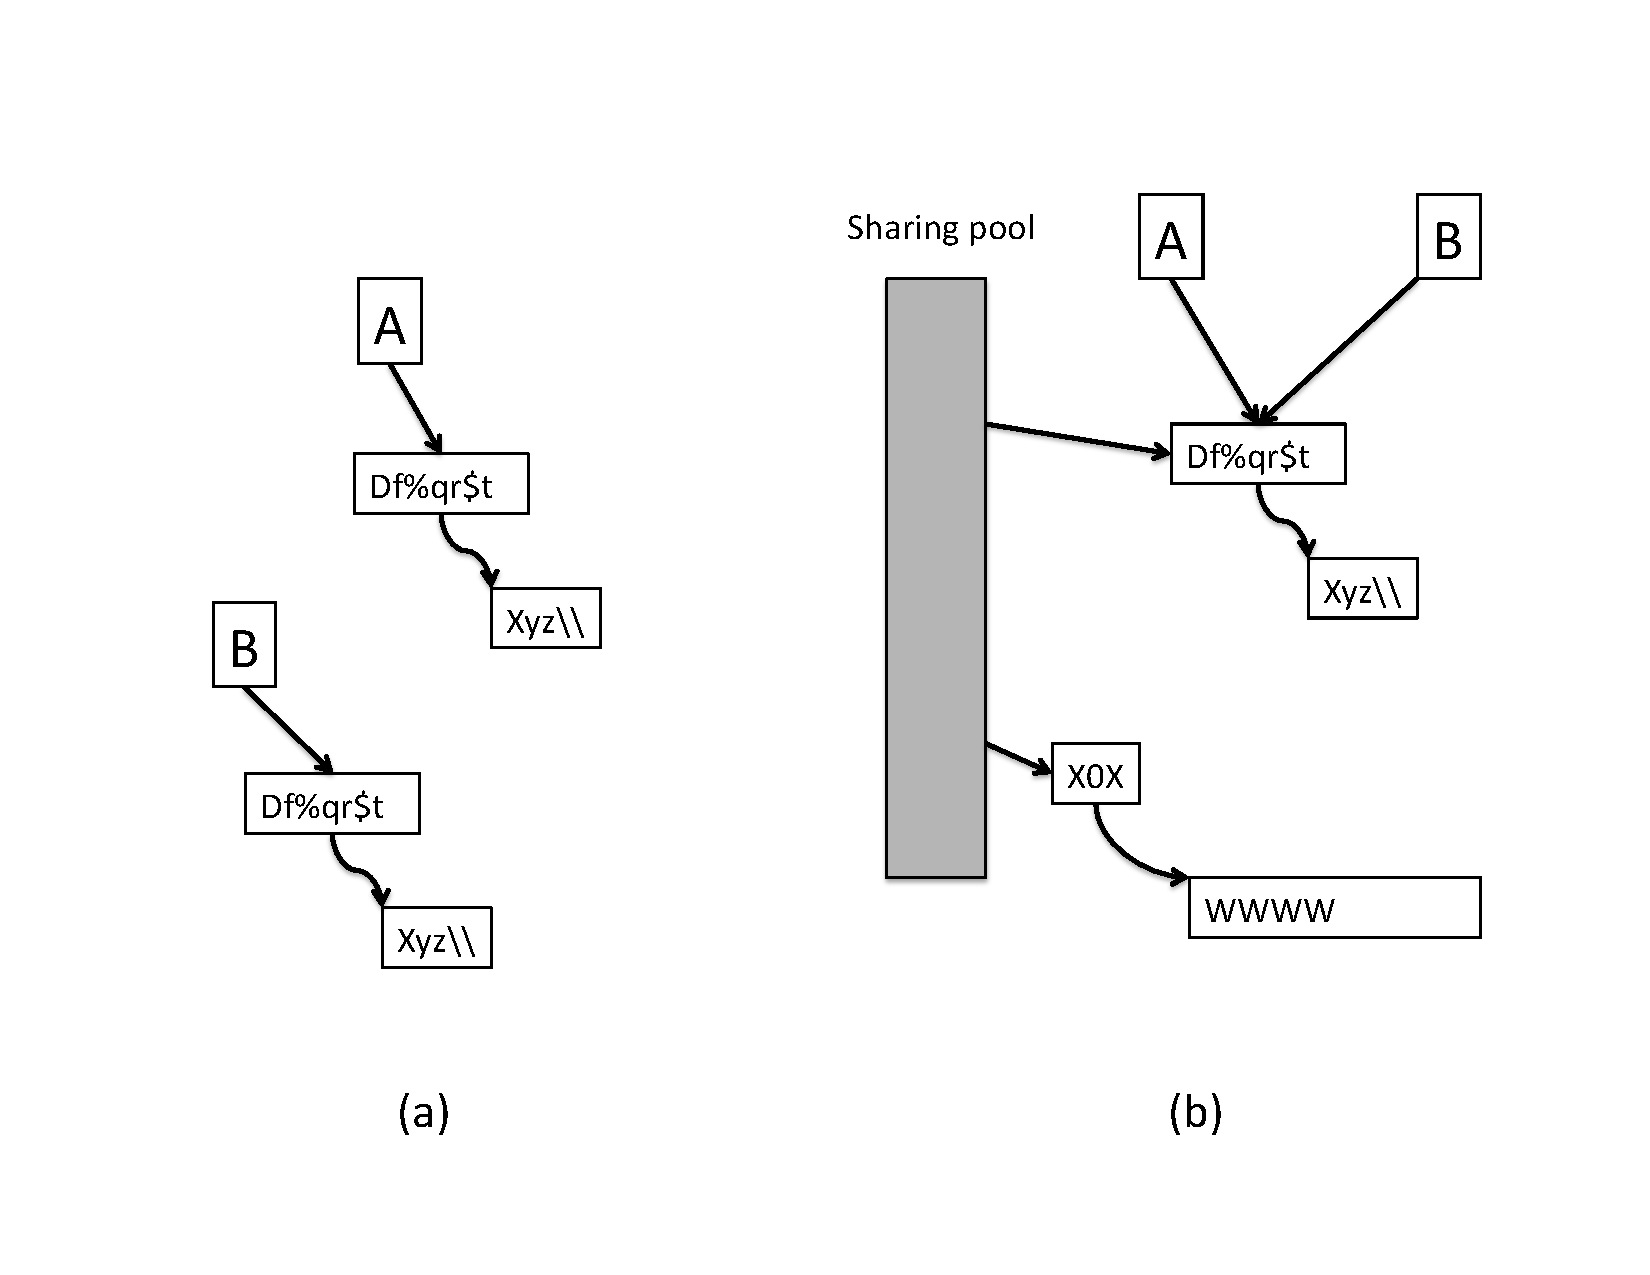
\includegraphics[width=.80\textwidth]{part2/Figures/chapter4/sharing-pool.pdf}
  \caption{(a) Objects A and B point to duplicate data. (b) Objects A and B
  share the same data, stored in a sharing pool.}
  \label{fig:sharing-pool}
\end{figure}

\callout{callout:sharing-pool}{Sharing Pool}{
A \emph{sharing pool} is a centralized structure that stores 
canonical data values that would otherwise be replicated in many objects.
A sharing pool itself is usually a some sort of hash table, although it
could be implemented in other ways.
}

The following
pseudo-code implements sharing a new object. 

\begin{shortlisting}
    share(newObject) { 
        if (sharingPool contains a copy of newObject) {
        	return copy of newObject;  
        } else {
            add newObject to sharingPool;
            return newObject;
        }
    }
\end{shortlisting}


There are several issues that you need to be aware of before using a sharing
pool.
\paragraph{Shared objects must be immutable.} If shared data is changed
during execution, you could get some strange results. For example, if you
change the data stored in A in Figure~\ref{fig:sharing-pool}(b), you will
inadvertently also change the value of B.

\paragraph{Sharing objects changes identity semantics.} You must be
careful to make sure that equality gives the same result, whether or
not objects are shared.
 
First, you cannot use == on objects that you want to share.
For example, \code{A==B} is false in Figure~\ref{fig:sharing-pool}(a) and true 
in Figure~\ref{fig:sharing-pool}(b), which can lead to very subtle bugs.
In general, you should not use == unless you really want to test for object
identity, in which case, you cannot share.
 
Second, you need to be careful that \code{equals} gives the same result,
whether or not there is sharing.  For strings and scalars, \code{equals}
compares string values, so sharing is safe. For more
general structures, \code{equals} and == are the same, unless \code{equals} has
been redefined.

\paragraph{Sharing pools should not be used if there is limited sharing.}
As can be seen in Figure~\ref{fig:sharing-pool}, a sharing pool itself adds
memory costs, possibly including additional per-entry costs. If there is not
much sharing, then you aren't really saving any memory to justify the extra
cost. In fact, you may be wasting memory. 

\paragraph{Shared objects no longer needed should be garbage collected.}
In Figure~\ref{fig:sharing-pool}(b), the sharing pool stores an object
that no one else is pointing to. Over time, the sharing pool can fill up with
garbage, that is, items that were once needed but not any more. If the
sharing pool is not purged of these unused items, you have a memory
leak, and can run out of memory.

Whether or not you need to deal with these issues depends on the kind of
sharing pool you use, and whether it's built-in or not. 

\section{Sharing Strings}

%Before storing a 
%To use a sharing pool, before storing a new
%\class{String}, first check the pool to see if it is already there. If it is,
%reuse it; otherwise, add the new string to the pool. 
%One catch is that if you end up adding many strings to
%the pool that are never reused, then you will waste memory, since the pool
%structure itself has overhead. So you need to have a good idea
%which strings are likely to have duplicate values.

 Since string duplication is so common, Java provides a built-in string pool
 for sharing \class{String}s, implemented by the native JVM and maintained in
 its internal \emph{perm space}. To share a \class{String}, you simply call the
 method \code{intern} on it. Then everything is taken care of automatically.
Since strings are immutable, sharing is safe. However, you should not
use == on shared strings.
  
In the \class{ConfigurationWithStaticProperties} example from
seciton~\ref{literals}, property
name duplication was eliminated, but not
property value duplication. Suppose there are many duplicated values, but you
don't know them at compile-time. The following code interns the property value
strings as they are read in, which eliminates duplication during execution.
\begin{shortlisting}
 
 class ConfigurationPropertiesWithInterning {
    void handleNextEntry() {
       PropertyName propertyName = getNextPropertyName(); 
       String propertyValue = getNextString().intern();
       propertyMap.put(propertyName, propertyValue);
    }
}
\end{shortlisting}

By calling \code{intern} on each newly created string,
if the string has not already been saved, it is added to the internal string
pool, and a pointer to it is returned. Otherwise, the new string is a
duplicate, and a previously saved string is returned.

Even though interned strings are not stored in the heap, they do incur extra
overhead, and native memory costs add up also.
Therefore, you need to be careful to intern strings only when you know that
 there would be expensive duplication otherwise. Fortunately, the JVM
garbage collects unused interned strings, so you won't get a memory leak.
 
 Indiscrimately interning strings wastes memory and can fill up the perm space,
 in which case you will get an error message:
\code{java.lang.OutOfMemoryError:PermGen Space}. 
There are command line arguments for adjusting the size of the perm space:
XX:PermSize=128m sets perm size to 128 megabytes, and -XX:MaxPermSize=512m sets
the maximum perm size to 512 megabytes.

 %    * Literal strings within the same class in the same package represent
%     references to the same String object. * Literal strings within different
 %    classes in the same package represent references to the same String
%     object. * Literal strings within different classes in different packages
 %    likewise represent references to the same String object. * Strings
 %    computed by constant expressions are computed at compile time and then
   %  treated as if they were literals. * Strings computed by concatenation at
    % run time are newly created and therefore distinct.
\section{Sharing Integers}

Java also has a sharing pool for \class{Integer}s, which is quite different
from the internal string pool. The \class{Integer} sharing pool stores all
\class{Integer}s in a specific range, from -128 to 128. It is initialized at
class load time. You can share \class{Integer}s in the pool by
using the \code{Integer.valueOf} method instead of the constructor for creating
new \class{Integer}s. For example, if you want to store \class{Integer}s
from 1 to 500 in an array, the best way to do this from a memory standpoint is:
\begin{shortlisting}
    for (int i = 1; i <= 500; i++) {
        numbers[i] = Integer.valueOf(i);
    }
\end{shortlisting}
For the first 128 numbers, \code{valueOf} returns an existing \class{Integer}
that can be shared. For the rest of the numbers, \code{valueOf} creates a new
\class{Integer}.

Calling \class{Integer.valueOf} incurs no extra overhead, since the
\class{Integer}s have already been created. So the \class{Integer} sharing
pool can be used freely without worrying about wasting memory or getting a
memory exception. The only precaution is you shouldn't use == on shared
\class{Integer}s.

You can change the size of the \class{Integer} sharing pool by setting a
command line parameter: -XX:AutoBoxCacheMax=<size>.

\section{Sharing Objects}

It is not unusual to find a huge number of small, immutable structures in the
heap that are copies of each other. This is data structure duplication, which is coarser
than string and \class{Integer} duplication, and it can be very costly.
To eliminate this kind of duplication, you need to implement an immutable
structure factory, that maintains a sharing pool.

Immutable data, that has a 
small number of values, that was highly duplicated, and it turned out the type itself had some 
fields in it, and it delegated its work to String, which of course is highly delegated, 
because it delegates its work to char array. So this was a fairly easy problem to fix by just 
introducing the shared immutable factory pattern to say I need a type object that matches this 
particular constant. If I have one already, then just give me back that otherwise, make a new one 
and put it in your pool, and we�ll share it. The one thing to keep in mind when implementing 
things like that, is to make sure you avoid any lifetime management issues, in particular, 
memory leaks.  You can also introduce a concurrency problem if you are not careful.


You can implement your own map using weak references. Go into tht pattern later. 
To make sure you avoid a memory leak. The downside of that is that there can be some pretty 
high per entry cost. Doing it yourself in Java.  Don�t know the native entry cost, but know 
the per entry in Java is pretty high. 



Common prefix???

5.7 Example: Caching Strings

Most bloated designs have multiple problems, as shown in this example.  (Quiz??)

Analysis of what�s wrong with this example.
So this was an example from one of the Lotus frameworks, from Sametime Gateway, and this 
was one piece of a session connection, and like all the other examples, it�s one piece of a 
data puzzle with other problems and other sources of costs. It was kind of a medium scale run. 
We saw that the biggest part of this data structure had sessions 110 of them. Each of them had 2 
StringBuffers, and that was taking the bulk of the space here.  We looked in to it, and they had 
quite a few different problems. We saw these StringBuffers sitting in the long lived heap, and 
thought, why would anyone store stringbuffers as permanent memory. Typically stringbuffers are 
used as temporaries. They have very aggressive storage allocation, kind of like the collectio
ns, 
with the thought in mind that you are going to grow them. You are going to be editing them.  
Typically, long-lived memory doesn�t have that problem. Typically, Strings in particular, you 
build them up, and then they are pretty stable. So it seems sort of strange. Usually 
StringBuffer
 is 40\% empty space, because it has a doubling algorithm for allocating them.
 The other strange thing was that they had 3 of them per session, and then there was the 
 question of whether they needed them at all. Turns out we looked at the code, and they had a 
 confluence of 3 different issues going on here. First of all, they had a somewhat delegated 
 design, and again, this was one of the consequences that delegated designs can have, where it 
 causes coding pattern to be duplicated. So in this case, for a completely different reason, 
 they had taken their session objects and split them into 3 parts. And they had some good design 
 reasons for doing that for some replication functionality they needed. But along with that, 
 they took a coding pattern that said that everytime they call toString on this thing for some 
 logging purpose, we�re going to save the contents of that String so that we don�t have to 
 recomputed it. That was really their main problem, that they didn�t realize how much space 
 they were 
taking 
up by saving this computation. And sometimes that�s indeed worth it. 
That you compute something and hold onto it.  In this case they realized they didn�t need to hold 
onto that much stuff. So in this case they had 3 problems. One is they were holding onto it, 
and it got multiplied by 3 because it was a delegated design. The second problem was they were 
holding onto it, and they may not need to. The third problem was they were going to hold onto it,
 
StringBuffer was the wrong thing to use.  In the end, they would have been better off 
trimming the StringBuffer, or just calling toString on it, and getting a shorter 
String out of it.



The JVM stores string literals in a \emph{string constant pool}. Since strings
are immutable, it is safe for the JVM to eliminate duplicates, and keep just
one copy of each literal string. In the following code, the JVM stores two
strings, \code{``Harry''} and \code{``Tom''} in the constant pool, and
\code{name1} and \code{name3} share the string \code{``Harry''}.
\begin{shortlisting}
class BunchOfStrings {
	String name1 = ``Harry'';
	String name2 = ``Tom'';
	String name3 = ``Harry'';
}
\end{shortlisting}

 

